\section{Experiments}
\label{experiments}


\subsection{Dataset}\label{dataset}
To train the model, we incorporated two different datasets Realistic Single Image Dehazing (\textit{RESIDE}) dataset \cite{bench} with  total number 18,200  images for training are consider and additionally the Real-world Video Dehazing dataset (\textit{REVIDE-indoor}) \cite{revid} with a total of 1697  images for training and 282 for testing. To infer the proposed model, we used various benchmarking datasets like Dense haze \cite{dense_haze}, NH haze \cite{nh_haze}, I haze \cite{i_haze} and O haze \cite{o_haze}. We split the training dataset into 80\% training and 20\% validation. In pre-processing, we resize input images into $128 \times 128$ and change the colour space to YCbCr. We used batch size $64$ for all of the images. 

\subsection{Training setup}\label{train_setup}

We used AdamW \cite{admw} rather than Adam optimizer, as we used weight normalization weight decay from AdamW will be a reasonable regularizer. The weights are initialized in uniform distribution as proposed by He et al. \cite{kaiming} initial biases were set to zero. The learning rate we consider for training the model is 0.0001 and the weight decay is $10^{-5}$. If the loss doesn't change for 7 epochs, then dynamically the learning rate will be reduced by a factor of 2.

After testing both $\mathcal{L}_1$ \eqref{eqn:l1_loss} and $\mathcal{L}_2$ losses \eqref{eqn:mse}, we choose $\mathcal{L}_2$ as our primary loss. The final loss function includes $\mathcal{L}_2$ loss, Frequency domain loss \eqref{eqn:fft}, and structural similarity loss \eqref{eqn:ssim_loss}, and metrics include PSNR \eqref{eqn:psnr} and SSIM \eqref{eqn:ssim} as shown in Fig  \eqref{tab:vis_loss_metric}.

% Please add the following required packages to your document preamble:
% \usepackage{graphicx}
\begin{figure}[h]
\caption{The training and validation plot. Blue (train) indicates training and orange (val) indicates validation. a) Loss, b) PSNR, c)SSIM}
\label{tab:vis_loss_metric}
\resizebox{\columnwidth}{!}{%
\begin{tabular}{lll}
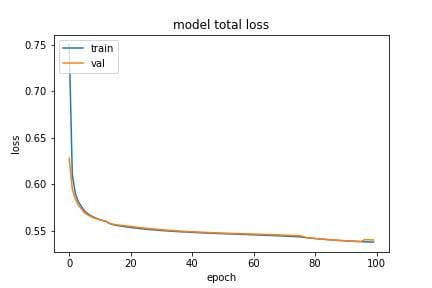
\includegraphics[height=14cm,width=16cm]{images/loss.jpg}& 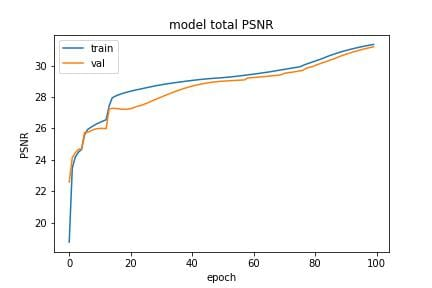
\includegraphics[height=14cm,width=16cm]{images/PSNR.jpg} & 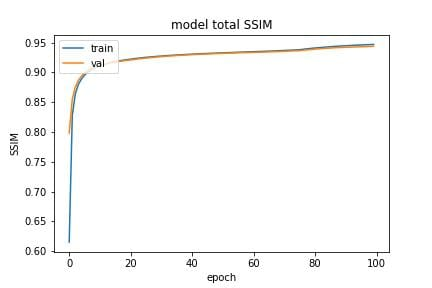
\includegraphics[height=14cm, width=16cm]{images/SSIM.jpg} \\
\multicolumn{1}{c} {\Huge{a) Loss}} & \multicolumn{1}{c}{\Huge{b) PSNR}} & \multicolumn{1}{c}{\Huge{c) SSIM}}
\end{tabular}%
}
\end{figure}

\subsection{Comparing results with other methods}
\label{comapring}
We computed metrics PSNR \eqref{eqn:psnr} and SSIM \eqref{eqn:ssim} on various real-world and synthetic images. We presented our results in  Table.~\eqref{tab:my-table} and Table. \eqref{tab:my-table1} with a detail analysis with existing methods.
\label{comparing}

\begin{table}[h]
\centering
\caption{The quantitative analysis of result  with respect to the existing  methods and our model on Dense-Haze, NH-Haze.
}
\label{tab:my-table1}
% \resizebox{\columnwidth}{!}{%
\begin{tabular}{cccccc}
\multicolumn{6}{c}{\textit{\textbf{Dense-Haze}}   \cite{dense_haze} }                                      \\ \hline
\textbf{Metric} & \textit{\textbf{Berman et al.}} \cite{prior1} & \textit{\textbf{AOD-Net}} \cite{aod} & \textbf{BPPNet} \cite{bppnet_sota} & \textit{\textbf{EDN-GTM}} \cite{sec_sota} & \textit{\textbf{Our}} \\ \hline
\textbf{PSNR (dB)} & 13.18 & 13.14       & 17.01       & 15.43          & \textbf{17.60} \\
\textbf{SSIM}      & 0.358 & 0.414       & 0.613       & 0.520          & \textbf{0.716} \\ \hline
\multicolumn{6}{l}{}                                                                     \\
\multicolumn{6}{c}{\textit{\textbf{NH-Haze}}  \cite{nh_haze}}                                           \\ \hline
Metric          & \textbf{He et al.}  \cite{he}            & \multicolumn{2}{c}{\textbf{AOD-Net} \cite{aod}}       & \textbf{EDN-GTM} \cite{sec_sota}         & \textit{\textbf{Our}} \\ \hline
\textbf{PSNR (dB)} & 16.62 & \multicolumn{2}{c}{15.40} & \textbf{20.24} & 18.93          \\
\textbf{SSIM}      & 0.523 & \multicolumn{2}{c}{0.569} & 0.718          & \textbf{0.746} \\ \hline
\end{tabular}%
% }
\end{table}
As exhibited in Table \eqref{tab:my-table}, the model performs near state-of-the-art in both PSNR and SSIM metrics on both datasetes \cite{i_haze, o_haze}. Whereas from Table \eqref{tab:my-table1}, our model outperforms existing methods in both PSNR and SSIM with the Dense-haze dataset \cite{dense_haze}. For the NH-Haze \cite{nh_haze} dataset, our model outperforms existing models in SSIM and the PSNR difference between our model and the existing model is 1.31dB. In both cases, EDN-GTM \cite{sec_sota} struggles in the SSIM metric, but our method gives a precise SSIM score because of the Structural similarity loss \eqref{eqn:ssim_loss}, see results in Fig (\ref{tab:Results}).
